\documentclass{article}
\usepackage{tikz}
\usetikzlibrary{graphs,graphdrawing}
\usepackage{caption}

\usepackage{multirow}
\usepackage{multicol}
\usepackage[framemethod=tikz]{mdframed}
\usepackage{lipsum}
\usepackage{tkz-graph}
\usegdlibrary{trees}
\usepackage{amsmath, amssymb}
\usepackage{pst-node}
\usepackage{blkarray}
\usepackage{amsmath, amssymb}
\usepackage{pst-node}

\usepackage[margin=2cm]{geometry}

\usepackage[utf8]{inputenc}
\begin{document}
	\section{Esercitazione 6}
	\subsection{Esercizio 1}
	
	Si supponga di volere modellare il comportamento di una semplice lampadina. Si consideri il tempo scandito in
	modo discreto (di secondo in secondo) e che i problemi che possono presentarsi siano i seguenti:
	
	\begin{enumerate}
		\item La lampadina può fulminarsi e smette di funzionare con probabilità 0.05.
		\item La lampadina può risultare troppo calda, per cui ha difficoltà ad accendersi. La probabilità che la lampadina si
		possa surriscaldare troppo vale 0.15 e che in tale situazione abbia probabilità 0.35 di accendersi.
	\end{enumerate}
Si supponga inoltre che il sistema (perfetto) di rilevazione degli errori che si intende utilizzare per verificare il corretto
funzionamento della lampadina indichi l’assenza di errori (good) o la presenza di errori (bad).
Modellare il problema mediante una catena di markov nascosta.

\textit{Per problemi di traduzione il testo è un po' ambiguo ma con "lampadina si
	possa surriscaldare troppo vale 0.15" si intende che la probabilità di diventare o rimanere surriscaldata è sempre 0.15 }

\begin{itemize}
\item	Quali sono gli stati?
\end{itemize}

\[ \Omega = { OK, \; HOT,  \; KO  }\]

\begin{itemize}
		\item Quali sono le possibili osservazioni?
\end{itemize}

\[
	\Sigma = { good, \; bad}
\]

\begin{itemize}
	\item Quali sono le distribuzioni di probabilità di cui abbiamo bisogno?
\end{itemize}

\begin{enumerate}
	\item Distribuzione iniziale di probabilità: \[\pi = (0, 0, 1)^T \] \\
	     Assumiamo che inizialmente la lampadina sia sempre funzionante
	     
	\item Matrice di transizione $A$ 
	\[
	A = 
	\begin{blockarray}{cccccc}
		& OK & HOT & KO \\
		\begin{block}{c(ccccc)}
			OK &	0.8 &  0.15   & 0.05   \\
			HOT &	0.8 &  0.15   & 0.05 \\
			KO &	0   &  0      & 1   \\
		\end{block}
	\end{blockarray}
	\]	
	
	\item Matrice di emissione delle osservazioni.
	
	\begin{mdframed}[hidealllines=true,backgroundcolor=blue!20]
		La matrice di emissioni delle osservazioni mi dice per ogni stato quali osservazioni posso emettere.
	\end{mdframed} 
		\[
	E = 
	\begin{blockarray}{cccccc}
		& Good & Bad \\
		\begin{block}{c(ccccc)}
			OK  &	1    &  0   \\
			HOT &	0.35 &  0.65   \\
			KO  &	0    &  1      \\
		\end{block}
	\end{blockarray}
	\]	

\pagebreak

\begin{itemize}
 \item  Qual è la rappresentazione grafica dell' HMM?
\end{itemize}
	\begin{center}
		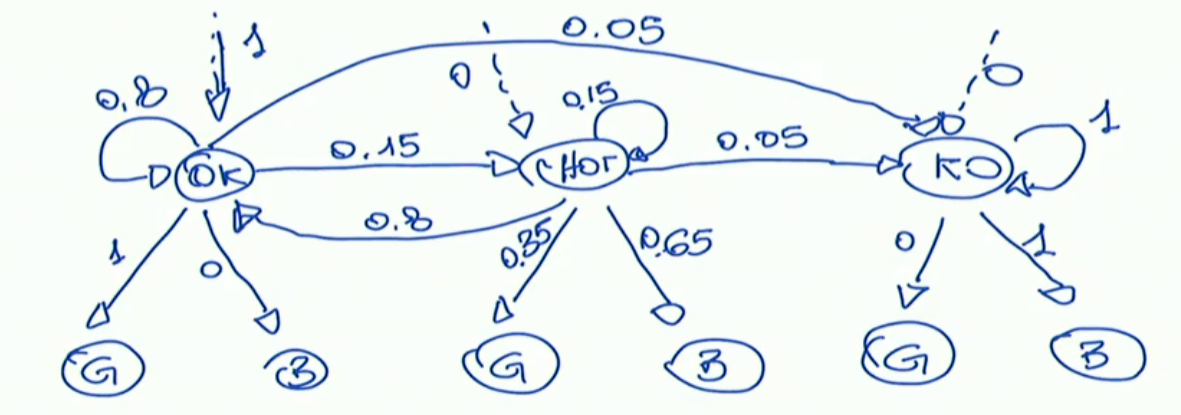
\includegraphics[width=14cm]{./immagini/hmm_es1.png}
	\end{center}
	
\end{enumerate}

\pagebreak
	\subsection{Esercizio 2}
	Dato un HMM caratterizzato da:
	\begin{itemize}
		\item Un insieme di stati $S = \{S_1, ..., S_k\}$
		\item Un insieme di osservazioni  $O = \{O_1, ..., O_m\}$
	\end{itemize}
	
	Quanti parametri sono necessari per definire un HMM?
	
	I parametri necessari sono:
	
	\[
		k + k^2 + km
	\]
	
\begin{itemize}
	\item $k$ rappresenta ciò che prima abbiamo chiamato $\pi$, ovvero il \textbf{vettore delle probabilità iniziali}. \\
	Sarà un vettore $\pi = [1, ..., k]$
	
	\item $k^2$ rappresenta la matrice di transizione fra gli stati, quella che prima abbiamo chiamato $A$.
	
	\item $km$ è una matrice che rappresenta le possibili osservazioni che uno stato può produrre, quella che priam abbiamo chiamato $E$.
\end{itemize}

L'unione di questi parametri ci consente di specificare un HMM

\pagebreak

\subsection{Esercizio 3}

Consideriamo questo HMM:

Vettore delle probabilità iniziali
\[P  = [0.5; 0.5];\]

Matrice di transizione $T$
\[
T = 
\begin{blockarray}{ccc}
	& S_1 & S_2 \\
	\begin{block}{c[cc]}
	S_1 &	0.3  &  0.7   \\
	S_2 &	0.4  &  0.6   \\
	\end{block}
\end{blockarray}
\]	

Matrice di emissione delle osservazioni  $O$
\[
O = 
\begin{blockarray}{ccc}
		& A & B \\
	\begin{block}{c[cc]}
	S_1 &	0.4  &  0.6   \\
	S_2 &	0.8  &  0.2   \\
	\end{block}
\end{blockarray}
\]	

\begin{itemize}
	\item Disegnare il modello probabilistico
\end{itemize}
	\begin{center}
	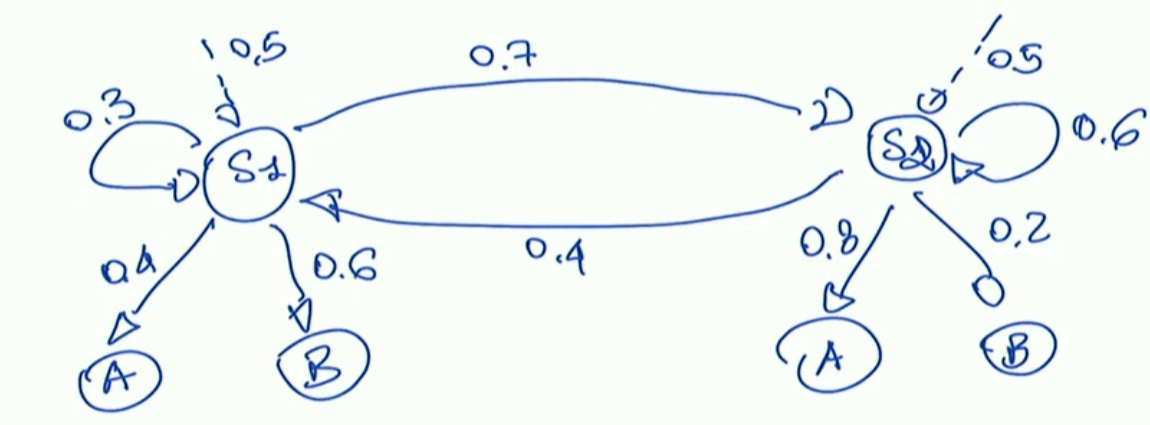
\includegraphics[width=14cm]{./immagini/hmm_es2.png}
\end{center}

\begin{itemize}
	\item Calcolare la probabilità della sequenza di stati
	\[
		S = \{ S_1, S_1, S_2, S_1, S_2\}
	\]
\end{itemize}

Avremo che la probabilità di una sequenza di stati è:
\[
P(S | \theta ) = \prod_{t = 1}^{|S|} T_{t, t + 1}
\]

Ovvero

\[
P(S_1, S_1, S_2, S_1, S_2) = 
P(S_1) \cdot 
P(S_1 | S_1) \cdot 
P(S_2 | S_1) \cdot 
P(S_1 | S_2) \cdot 
P(S_2 | S_1) 
\]

Sostituendo $P(S_1)$ prendendolo dal vettore delle probabilità iniziali e gli altri valori prendendoli dalla matrice di transizione otteniamo:

\[
 = 0.5 \cdot 0.3 \cdot 0.7 \cdot 0.4 \cdot 0.7 = 0.0294
\]

\pagebreak

\begin{itemize}
	\item Calcolare la probabilità della sequenza di osservazioni
	\[
	E = \{ A, A, B, A, A\}
	\]
	data la sequenza degli stati
	\[
	S = \{ S_1, S_1, S_2, S_1, S_2 \}
	\]
\end{itemize}

La richiesta è quella di calcolare della sequenza di osservazioni $E$ non solo dati i parametri iniziali ma anche data una sequenza di stati $S$.

\[
	P(E | \theta, S) = \prod_{i=1}^{|E|} P(e_{t} | s_i, \theta)
\]

Ovvero:

\[
 = P(A | S1) \cdot P(A | S1) \cdot P(B | S2) \cdot P(A | S1) \cdot P(A | S2)
\]

\[
	= 0.4 \cdot 0.4 \cdot 0.2 \cdot 0.4 \cdot 0.8 = 0.01024
\]

\begin{itemize}
	\item Calcolare la joint likelihood della sequenza di osservazioni 	\[
	E = \{ A, A, B, A, A\}
	\]
	e la sequenza degli stati
	\[
	S = \{ S_1, S_1, S_2, S_1, S_2 \}
	\]
\end{itemize}

La richiesta è quella di trovare
\[
P(E, S | \theta) = P(E | S, \theta) \cdot P(S | \theta) = 
\]

\[
 = 0.01024 \cdot 0.0294 = 0.000301056
\]

\pagebreak

\subsection{Esercizio 4}

Si consideri il seguente HMM che modella la probabilità di avere una annata
molto calda/fredda, osservando la chioma degli alberi. Il modello HMM è
caratterizzato dalle seguenti distribuzione di probabilità discrete:

\[\pi = [0.5, 0.5] \]


\[
T = 
\begin{blockarray}{ccc}
	& H & C \\
	\begin{block}{c[cc]}
		H &	0.7  &  0.3   \\
		C &	0.4  &  0.6   \\
	\end{block}
\end{blockarray}
\]	

\[
O = 
\begin{blockarray}{ccc}
	& S & L \\
	\begin{block}{c[cc]}
		H &	0.4  &  0.6   \\
		C &	0.8  &  0.2   \\
	\end{block}
\end{blockarray}
\]	


\begin{itemize}
	\item Effettuare il task di filtraggio utilizzando le osservazioni ${S, S, L}$
\end{itemize}


\begin{mdframed}[hidealllines=true,backgroundcolor=blue!20]
	Il task di filtraggio è composto da due sottopassi: il passaggio di predizione, dove faccio evolvere il modello da un tempo $t$ al tempo successivo e poi ho la fase di aggiornamento dove vado a considerare l'osservazione per aggiornare la predizione.
\end{mdframed} 

Predizione da $t_0$ a $t_1$:

\[
	P(S_1 | S_0) = \sum_{s_i \in S_0} P(S_1 | s_i) \cdot P(s_i)
\]

Dove $P(S_1)$ indica la distribuzione probabilità dello stato del sistema al passo 1

\[
 = (0.5 \cdot <0.7 ; 0.3> ) + (0.5 \cdot <0.4 ; 0.6> )
\]

Le due espressioni significano:
\begin{enumerate}
	\item  inizialmente sei nello stato $HOT$ con probabilità 0.5, fai "un salto in avanti" con probabilità 0.7 di rimanere in $HOT$ e con probabilità 0.3 di andare in $COLD$.
\end{enumerate}

\begin{enumerate}
	\item  inizialmente sei nello stato $fpòd$ con probabilità 0.5, fai "un salto in avanti" con probabilità 0.4 di andare in $HOT$ e con probabilità 0.6 di rimanere in $COLD$.
\end{enumerate}


\[
= <0.35 ; 0.15>  + <0.2 ; 0.3> = <0.55 ; 0.45>
\]

Effettuiamo il passaggio di aggiornamento sapendo che all'istante $t_1$ abbiamo osservato una chioma $S$:

Dobbiamo quindi calcolare:

\[
P(S_1 | s) = \alpha \cdot P(s | S_1) \cdot P(S_1)
\]

In concreto $P(S_1 | s)$ significa prendere la predizione ed aggiornarla rispetto a ciò chè è stato osservato

$P(s | S_1)$ è la distribuzione di probabilità di emettere l'osservazione small, indipendentemente dal fatto che $S_1$ sia $HOT$ oppure $COLD$: prendiamo quindi la colonna dell'osservazione $S$ dalla tabella $O$.

\[
= \alpha \cdot <0.4; 0.8> \cdot < 0.55 ; 0.45 > =
\]

\[
= \alpha \cdot <0.22; 0.36> = <0.379; 0.621>
\]

Concludiamo quindi che $S_1 = <0.379; 0.621>$.

\pagebreak

\begin{itemize}
	\item Effettuiamo la predizione da $t_1$ a $t_2$
\end{itemize}

Avremo che nella fase di predizione:

\[
P(S_2 | S_1) = \sum_{s_i \in S_1}  P(S_2 | s_i) \cdot P(s_i)
\]

Ovvero

\[
 = (0.379 \cdot <0.7 ; 0.3> ) + (0.621 \cdot <0.4 ; 0.6> ) = 
\]

Dove 0.379 e 0.621 sono le nuove probabilità per $HOT$ e $COLD$ ottenute in precedenza.


\[
= <0.265 ; 0.1137> + <0.2484 ; 0.3726>  = <0.5134 ; 0.4863>
\]

A questo punto sappiamo che all'istante due abbiamo osservato una chioma $S$, per cui andiamo ad aggiornare la stima di $S2$

\[
P(S_2 | s) = \alpha \cdot P(s | S2) \cdot P(S_2)
\]

Ovvero

\[
P(S_2) = \alpha \cdot < 0.4; 0.8 > \cdot  < 0.5134 ; 0.4863>
\]

\[
P(S_2) = \alpha \cdot < 0.20536; 0.38904 > 
\]

Normalizzando otteniamo che $\alpha = 0.5944$, da cui
concludiamo che 

\[
P(S_2) = <0.3454; 0.6545>
\]

\begin{itemize}
	\item Effettuiamo la predizione da $t_2$ a $t_3$
\end{itemize}

Sappiamo che:

\[
P(S_3 | S_2) = \sum_{s_i \in S_2} P(S_3 | s_i) \cdot P(s_i)
\]

Ovvero:
\[
 (0.3454 \cdot <0.7 ; 0.3> ) + (0.6545 \cdot <0.4 ; 0.6> ) = 
\]

\[
	<0.24178 ; 0.10362> + <0.2618 ; 0.3927>  = <0.50; 0.50> 
\]

A questo punto sapendo che all'istante tre abbiamo osservato una chioma $l$, per cui andiamo ad aggiornare la stima di $S_3$

\[
P(S_3 | l) = \alpha \cdot P(l | S_3) \cdot P(S_3)
\]

\[
 = \alpha \cdot <0.6; 0.2> \cdot <0.5; 0.5> =
\]

\[
= \alpha \cdot <0.6; 0.2> \cdot <0.5; 0.5> =
\]

\[
= \alpha \cdot <0.3; 0.1>
\]

Normalizziamo utilizzando $\alpha = 2.5$ e otteniamo che $S_3 = <0.75; 0.25>$

\pagebreak

\begin{itemize}
	\item Tenendo in considerazioni il filtrato a 3 step, quale è la probabilità che il 5° anno sia "hot"?
\end{itemize}

A questo punto non avendo più osservazioni dobbiamo solo fare l'evoluzione temporale in avanti.

Dobbiamo quindi moltiplicare per $T^2$, perché mancano gli ultimi due passi:

\[
P(S_5 | s, s, l) = <0.75; 0.25> \cdot T^2
\]

\[
 = < 0.5878; 0.4122> 
\]

\end{document}


